% 中文平行版阶段报告二：结构、数字、图表与 stage_report_2.tex 完全一致。
% 编译（LM2，两遍，目录 docs/report/stage_report_2/）：export PATH=/data6/jinxinhao/texlive/2026/bin/x86_64-linux:$PATH
%   xelatex stage_report_2_zh.tex && xelatex stage_report_2_zh.tex
% 全部数字于 2026-10-01 从 artifacts 重新导出核验（runs/analysis/report2_numbers.txt）。
\documentclass[11pt]{article}
\usepackage[margin=1in]{geometry}
\usepackage{amsmath,amssymb}
\usepackage{booktabs}
\usepackage{multirow}
\usepackage{graphicx}
\usepackage{xcolor}
\usepackage{xeCJK}
\setCJKmainfont{FandolSong-Regular}[
  Extension = .otf, BoldFont = FandolSong-Bold,
  AutoFakeBold = 2.2, AutoFakeSlant = 0.2]
\setCJKsansfont{FandolHei-Regular}[Extension = .otf, AutoFakeBold = 2.2]
\renewcommand{\figurename}{图}
\renewcommand{\tablename}{表}
\renewcommand{\abstractname}{摘要}
\renewcommand{\refname}{参考文献}
\usepackage[hidelinks]{hyperref}
\emergencystretch=3em

\title{\bfseries Dead 检测瓶颈的两条攻坚路线：\\
检测优先架构未能兑现，$2\times$ 分辨率能换来 Dead，但明码标价\\[6pt]
\large 阶段报告二（课程项目 bdd26）}
\author{}
\date{2026 年 10 月 1 日}

\begin{document}
\maketitle

\begin{abstract}
阶段报告一把 PanNuke 上 \textbf{Dead}（凋亡）类的缺陷定位在\textbf{检测}：38.5\% 的 Dead
真值核没有任何重叠预测，且该缺陷挺过了我们测试的全部损失级与数据级干预，横跨三种稠密解码
器架构。当时留下两条未经检验的出路：文献中 Dead 数字最强的\emph{检测优先}架构家族，以及
\emph{工作分辨率}。本报告在同一严格协议下（官方 3-fold、last checkpoint、仅验证折调参、
伪影感知的 Dead 口径）检验了这两条路线。\textbf{A 线（负结果）}。发布分折权重的
KongNet——一个六头 CenterNet 式检测器，其折映射先经实证厘清——在验证折调优的解码下仅得
0.346 mPQ，比\emph{最弱}的稠密解码器还低 11 个点；其轮廓切割通道在 40$\times$ 下净有害
（每个 checkpoint 的最优解都把它关掉）；相触的同类核被并合（merged 率 0.12--0.18，watershed
解码器为 0.04--0.05）；内部 Dead 漏检\emph{更高}（0.50 对 0.35）；论文的 Dead $F_c$ 0.59
在严格协议下降至 0.34。LKCell-L——我们能找到的最强发布分折权重——比论文均匀低约 0.015，
且在同等条件下是\emph{更好的分割器、更差的分型器}（bPQ $+0.008$，Dead PQ $-0.022$）：
架构优势不能转化为 Dead 或分型收益。\textbf{B 线（一项明码标价的交换）}。把工作分辨率
单变量地倍增到 512\,px 后，全部预注册 Dead 端点转正（内部 Dead 漏检 $0.35\!\to\!0.25$），
代价是均匀的 bPQ 税 $-0.026$。误差分析否定了降采样假说（即"把 512 的预测图缩回 256 时
丢了边界"），把税款的主要来源追到一个隐藏混淆变量：watershed 解码中的\emph{固定像素
单位常数}（最小目标面积、Sobel 孔径）在 $2\times$ 下以原生像素为单位悄然放松。预注册
修复——按分辨率因子缩放这些常数——收回 mPQ/bPQ/mPQ$^+$ 代价的 50--87\%，Dead 增益保留
并略有放大；随后一个仅用验证折选择的后处理杠杆（同类实例合并 $+$ 边缘细条丢弃）在
$3{\times}3$ 分裂$\times$种子网格的全部 9 个 run 上都取得严格的测试集改进。该网格的预注册
种子噪声判定：\emph{代价}种子稳健（最大种子标准差的 $4.7$--$5.3\times$，逐 run 同号）；
\emph{Dead 增益}脆弱（逐种子 Dead 标准差的 $0.4$--$0.7\times$，有一个分裂的种子均值变号）。
终局：$-0.008$ mPQ / $-0.005$ bPQ 换 $-0.069$ 内部 Dead 漏检、$+0.034$ Dead $F_c$ 与
mPQ$^+$ 持平——不是默认的胜利，而是一次明码标价的交换。结论：Dead 缺陷不是某个架构家族
的伪影——更多像素确实买到了真实的检测收益，而把新分辨率下显形的东西切开、并判对类型，
仍是悬而未决的那一半；像素单位解码常数是一等混淆变量，任何分辨率研究都必须对其加以
控制。
\end{abstract}

\section{引言}
\label{sec:intro}

阶段报告一以一个闭环的诊断收尾：在 PanNuke~\cite{gamper2019pannuke} 上，Dead（凋亡小体）
类输在\emph{检测}而非分类——漏检 Dead 核中 83\% 的前景头毫无响应，类型分支却已给出
P(Dead)$\approx$0.26；病理 VLM 重分类、免训练找回、损失重加权、copy-paste 增强与上下文内
合成全部无效或有害；且该缺陷为我们评测的三种稠密解码器架构（ViT-L/16、全分辨率
ResNet-50、ConvNeXt 解码器）所共有。两条假说由此悬而未决，本报告在预注册、噪声标定的协议
下将它们一并收官：

\begin{enumerate}
\item \textbf{架构（A 线）}：失败源于\emph{稠密解码器}（前景 $+$ watershed）本身。先预测
逐类质心、再围绕质心组装掩膜的检测优先设计，在文献中报出远超稠密模型的 Dead 数字
（KongNet~\cite{lv2025kongnet}：逐核 Dead $F_c$ 0.59，而我们的稠密模型在严格解码下仅
0.23--0.36）。若该优势在同等评测条件下成立，Dead 缺陷就有架构层面的解。我们端到端检验
KongNet 的发布分折权重——先实证厘清其未记载的折映射——并在同一管线中复评 CellViT 家族
中发布分折权重的最强者 LKCell-L~\cite{cui2024lkcell}。
\item \textbf{分辨率（B 线）}：失败反映的是 256\,px 工作分辨率。Dead 核小（中位面积
107\,px，其它类 368\,px），内部 Dead 核的漏检率达 31\%，且面积已达 $\geq$256\,px 的 Dead
核仍有 17\% 漏检——无论解码器为何，
更多像素都应改善检测。我们把 CellViT-UNI 配方的工作分辨率倍增（单变量改变），然后顺着误差
线索一路追下去：初局的均匀 bPQ 税、推翻显然解释的机制诊断、预注册的解码修复、仅验证折选择
的后处理杠杆，以及在最后一批 run 落地之前就写定判定规则的 $3{\times}3$ 分裂$\times$种子
网格。
\end{enumerate}

贡献如下：

\begin{enumerate}
\item \textbf{检测优先架构的严格协议判定}（\S\ref{sec:lineA}）：KongNet 发布分折权重在
其最优验证折解码下比最弱稠密解码器低 11 个 mPQ 点，把相触的同类核并在一起，漏掉\emph{更
多}内部 Dead 核；论文 Dead $F_c$ 0.59 不复现（严格口径 0.34）。LKCell-L 在同等条件下分割
更好、分型更差。可推广的教训：迄今发表的 Dead 优势反映的是评测配方与分割--分型的取舍，
而非真正更好地检测出了 Dead。
\item \textbf{分辨率在核解码中的机制研究}（\S\ref{sec:mechanism}--\ref{sec:du2}）：
$2\times$ 的 bPQ 税随尺寸单调、不按类别分布；匹配核的边界质量不变；主因是 watershed 解码
硬编码的两个像素单位常数（目标面积下限、Sobel 孔径），分辨率倍增时它们以原生像素为单位
放松。按因子缩放（$du2$）收回聚合代价的 50--87\%。据我们所知，这一混淆变量在细胞核分割
文献中无人记载，而它适用于\emph{任何}建立在 HoVer-Net 后处理栈上的管线。
\item \textbf{$2\times$ 分辨率的预注册、全复现、明码标价刻画}（\S\ref{sec:lever}--\ref{sec:final}）：
仅验证折选择的杠杆（同类合并 $+$ 细条丢弃，常数冻结）在全部 9 个网格 run 上严格改进 $du2$
手臂；$3{\times}3$ 种子网格把稳健的代价与脆弱的 Dead 增益区分开；终局以 mPQ/bPQ 单位为
每一项 Dead 改进标出价格。
\item \textbf{两项评测方法学结果}：发布权重的 KongNet 折映射可以仅凭记忆效应复原（训练
折检测 F1 优势 $\geq$0.13，不使用任何测试折信息）；LKCell-L 的论文--严格差距是\emph{均匀}
的（每项头部指标约 $-0.015$）——这是协议转换而非管线错误的标志，也是继报告一 HoVer-NeXt-T
之后第二个配方差距超过排行榜典型间距的发布模型。
\end{enumerate}

所有结果来自同一代码库与同一逐位一致的评测器；本报告的全部表格数字于 2026-10-01 从留存的
预测 artifacts 重新导出（脚本 \texttt{scripts/report2\_numbers.py}，提取结果随 run
artifacts 存档）。

\section{相关工作}
\label{sec:related}

\paragraph{稠密解码器家族。}HoVer-Net~\cite{graham2019hovernet} 确立了核概率 / 水平--垂直
/ 类型的三头分解与 watershed 解码，CellViT~\cite{horta2024cellvit} 全盘继承；
HoVer-NeXt~\cite{hovenext} 与 LKCell~\cite{cui2024lkcell} 是近年的变体。报告一已证明整个
家族共有 Dead 检测缺陷。

\paragraph{检测优先与点预测模型。}质心/热图式检测器可上溯至 StarDist 与 CenterNet 类设
计；KongNet~\cite{lv2025kongnet}（六头 EfficientNetV2-L：逐类热图 $+$ 回归 $+$ 分割/轮廓
通道）报出文献中最强的逐核 Dead $F_c$（0.59）并发布分折权重——这使它成为 A 线的正确检验
对象：主张具体、可查证，且直接承载"检测优先修复 Dead"这一假说。PromptNucSeg~\cite{promptnucseg}
与 CellVTA 代表提示/适配器分支，其发布权重的同一复评已排队（\S\ref{sec:status}）。

\paragraph{细胞核分割中的分辨率。}更高的输入或工作分辨率是常青杠杆（512\,px 的
CellViT-SAM-H、LKCell 的多尺度大核、HoVer-NeXt 的金字塔），但已发表的消融比较的是端到端
配置，而非把分辨率作为变量、把解码问责到底。与我们发现最接近的先声是经典尺度空间文献：
watershed 种子与形态学下限都是像素单位算子，其有效尺度随图像分辨率变化——而据我们所知，
在学习式细胞核分割管线中，这一事实从未被当作混淆变量指出；这些常数正是在 HoVer-Net 发布
的后处理代码中被原封不动继承下来的。

\section{实验设置}
\label{sec:setup}

\paragraph{协议（与报告一相同）。}PanNuke 折 1--3，官方划分（train/val/test $=1/2/3$、
$2/1/3$、$3/2/1$）；自行训练的 run 取 last checkpoint，复评模型取发布分折（验证折选出）
权重；任何环节不在测试折上调参；组织平均 mPQ/bPQ 出自逐位一致的评测器；TTA（8 个二面体
视图，HV 通道重映射）单独报告。Dead 端点按报告一的四种口径报告：官方 Dead PQ、去 Uterus
Dead PQ（官方逐类 PQ 只对含该类的图像取平均，而折 3 含 34 张所有模型都接近零分的 Uterus
图）、逐核 Dead $F_c$（12\,px 质心匹配）与内部（非贴边）Dead 漏检率。

\paragraph{发布权重复评规则（A 线）。}(1) 发布权重的折映射必须不经测试折确定：对 KongNet，
我们把每个 checkpoint 跑在所有\emph{训练}折的 200 图子样本上，从记忆对角线读出映射
（\S\ref{sec:kongnet}）。(2) 一切解码阈值仅在验证折上调优，网格扩展到最优被夹住为止；测试
折以冻结常数只跑一次。(3) 移植解码器的类别通道语义仅在训练折上核验（配对混淆对角
$\geq$0.97）。LKCell-L 以其发布配置（归一化、256\,px 解码）原样通过共享管线。

\paragraph{$2\times$ 工作分辨率（B 线）。}与 CellViT-UNI 完全相同的配方，工作分辨率倍增
到 512：增强之后双线性上采样图像、最近邻上采样标签；预测在 512 上做后处理、降采样到 256
交给标准评测器（逐实例类型概率表在模型分辨率上计算）。单变量改变。$du2$ 指
\S\ref{sec:du2} 的解码修复，\emph{杠杆}指 \S\ref{sec:lever} 的后处理。种子网格为
3 分裂 $\times$ 种子 \{19, 1, 2\}；基线种子 1/2 只在分裂 1 上存在（报告一），因此种子标准
差在分裂 1 上完整填充，并逐分裂报告。

\paragraph{噪声标定（沿用，且已两度验证）。}同一 CellViT-UNI 配方的种子标准差：mPQ
0.0021，Dead PQ 0.0074（分裂 1）；Dead 的图像 bootstrap CI 半宽 0.02--0.03。判定规则：
单种子 Dead 变化低于 $\sim$0.01--0.015 视为噪声；一切干预判定都是多 run 声明，配对、按
组织分层的图像 bootstrap 95\% CI；决策只在验证折上做。B 线的种子噪声判定在最后一批网格
run 落地前预注册（\S\ref{sec:grid}）。

\section{A 线：严格协议下的检测优先架构}
\label{sec:lineA}

\subsection{KongNet：折映射、最优解码与一个决定性的负结果}
\label{sec:kongnet}

\paragraph{资产与折映射。}KongNet 发布的分折权重
\texttt{KongNet\_PanNuke\_\allowbreak\{1,2,3\}.pth}
（1.769 亿参数，tf\_efficientnetv2\_L 编码器 $+$ 六个 SMP 解码器：一个整体头 $+$ 五个逐类
头，各含热图/分割/轮廓通道）没有附带任何折文档。把三个 checkpoint 全部跑在每个\emph{训
练}折的 200 图子样本上，得到干净的记忆对角线（合并检测 F1，12\,px 质心配对）：checkpoint
$k$ 在训练折 $k$ 上以 0.905/0.944/0.912 胜出，对两个 held-out 折优势 $\geq$0.13——
\texttt{\_k.pth} 即官方分裂 $k$，全程未用任何测试折信息。类别通道语义在训练折上核验
（配对类别一致率 0.97--0.99，Dead 对角干净）。

\paragraph{轮廓切割在 40$\times$ 下净有害。}发布推理配方把实例组装为逐类"分割减轮廓"掩
膜。我们在验证折上扫了两个解码阈值（网格两次扩展直至最优被夹住）。每个 checkpoint 的最优
解都\emph{完全关闭}轮廓切割（轮廓阈值 1.0）：checkpoint 1 上，关闭切割使验证 mPQ
$0.331\!\to\!0.345$、bPQ $0.457\!\to\!0.473$。仓库的轮廓阈值 0.3 配方在此尺度上过度切
核；切割关闭后，解码退化为朴素的逐类连通域。

\begin{table}[t]
\centering\small
\caption{严格协议架构总表（3 分裂均值，无 TTA，last/发布分折 checkpoint，验证折调优解
码）。Dead 端点：官方 PQ、去 Uterus PQ、逐核 $F_c$、DQ$^+$、内部 Dead 漏检（无匹配预测的
非贴边 Dead 真值占比；逐分裂速率均值）。HoVer-NeXt-T（报告一：0.458 mPQ / 0.637 bPQ /
0.136 Dead PQ）此处缺 artifact 导出的 Dead 列。LKCell-L 论文行照原文。}
\label{tab:arch}
\begin{tabular}{lcccccccc}
\toprule
模型 & mPQ & bPQ & mPQ$^+$ & \shortstack{Dead\\PQ} & \shortstack{Dead\\$-$Uterus} & \shortstack{Dead\\$F_c$} & \shortstack{Dead\\DQ$^+$} & \shortstack{内部 Dead\\漏检} \\
\midrule
KongNet（严格）   & .3460 & .4706 & .3472 & .053 & .070 & .344 & .232 & .520 \\
HoVer-Net（自训） & .4564 & .6613 & .4430 & .127 & .152 & .230 & .275 & .404 \\
LKCell-L（严格）  & .4923 & .6729 & .5235 & .154 & .201 & .382 & .418 & .347 \\
\quad 论文        & .508 & .685 & --- & .172 & --- & --- & --- & --- \\
CellViT-UNI（自训）& .4995 & .6653 & .5178 & .176 & .218 & .359 & .396 & .372 \\
\midrule
x2 $+$ du2          & .4894 & .6583 & .5157 & .183 & .226 & .395 & .424 & .302 \\
x2 $+$ du2 $+$ 杠杆 & .4910 & .6608 & .5171 & .183 & .227 & .393 & .422 & .302 \\
\bottomrule
\end{tabular}
\end{table}

\paragraph{测试判定。}表~\ref{tab:arch} 上块：冻结最优解码后，KongNet 得到 \textbf{0.346
mPQ / 0.471 bPQ}——比最弱的稠密解码器低 11 个 mPQ 点、17--19 个 bPQ 点——且全部预注册
Dead 端点失
败：官方 Dead PQ 0.053（稠密 0.127--0.176），去 Uterus 0.070，内部 Dead 漏检 0.50，
\emph{高于} CellViT-UNI 的 0.354 与 HoVer-Net 的 0.413（共享分裂 1+3 框架）。只有逐核
Dead $F_c$ 处于中游（0.344）。误差形态给出了答案：\emph{相触的同类核被并合}。merged-GT 率
逐分裂 0.121--0.175（CellViT-UNI 0.044--0.045，HoVer-Net 0.048--0.050）；轮廓切割关闭
后解码完全无法分离相触实例，而重新打开它损失更大。这正是报告一记录的核碎裂（karyorrhexis）
Dead 簇的失败几何（merged Dead 的 73--82\% 与另一个 Dead 相触）：Dead 缺陷是\emph{实例分
离}问题，不是检测密度问题——一个能找到 Dead 核却切不开碎片簇的检测器，什么也换不成 Dead
PQ。KongNet 论文的 Dead $F_c$ 0.59（其解码、其评测）在验证折调优解码下不再成立；A 线以
负结果关闭。

\subsection{LKCell-L：均匀的论文差距与"分割--分型"不可兑换}
\label{sec:lkcell}

LKCell-L（UniRepLKNet-S 编码器、RepLK 解码器、CellViT 三头）是 CellViT 家族中发布分折
权重的最强模型（论文：0.508 mPQ / 0.685 bPQ / 0.172 Dead PQ）。我们将其发布分折
\texttt{model\_best} checkpoint 跑过共享管线（其归一化、其 256\,px 解码、无 TTA）：

\begin{itemize}
\item \textbf{论文差距是均匀的}：严格 0.4923/0.6729/0.154，对照发表 0.508/0.685/0.172
——每项头部指标 $-0.016$/$-0.012$/$-0.018$。折或归一化错误会把指标砸穿，而均匀偏移是协议
转换（checkpoint 选择、解码、TTA 配方）的标志。照实记录；这一差距仅凭论文无法进一步
归因。
\item \textbf{同等条件下无 Dead 增益}：对照我们的 CellViT-UNI 基线（表~\ref{tab:arch}），
LKCell-L mPQ $-0.007$、Dead PQ $-0.022$，而 bPQ $+0.008$、mPQ$^+$ $+0.006$。分解：它
\emph{找} Dead 核更准（Dead $F_c$ 0.382 对 0.359；内部 Dead 漏检 0.347 对 0.372），但检
出的 Dead 核仍过不了类型配对——更好的检测换不成更好的 Dead PQ。与 KongNet 同向：匹配协议
下，一般性的架构优势不转化为 Dead 或分型收益。
\end{itemize}

值得注意的是，我们最贵的手臂（x2$+$du2$+$杠杆）在 mPQ 上与严格 LKCell-L 打平（0.4910 对
0.4923），却赢下全部 Dead 端点（内部 Dead 漏检 0.302 对 0.347；Dead $F_c$ 0.393 对
0.382；Dead DQ$^+$ 0.422 对 0.418）。

\section{B 线：$2\times$ 工作分辨率}
\label{sec:lineB}

\subsection{B1：全部 Dead 端点转正，附一笔均匀的 bPQ 税}
\label{sec:b1}

\begin{table}[t]
\centering\small
\caption{B1 初始结果（分裂 1，TTA）：$2\times$ 分辨率对照 3 种子基线（括号为种子标准
差；$\Delta$ 带配对、按组织分层的图像 bootstrap 95\% CI；逐类行只列 $\Delta$）。}
\label{tab:b1}
\begin{tabular}{lccc}
\toprule
指标 & 基线（3 种子） & x2（种子 19） & $\Delta$ [95\% CI] \\
\midrule
mPQ                & .4979 (.0032) & .4800 & $-$.0180 [$-$.0238, $-$.0122] \\
bPQ                & .6708 (.0018) & .6447 & $\mathbf{-}$.0261 [$-$.0308, $-$.0219] \\
Dead PQ            & .1429 (.0054) & .1614 & $\mathbf{+}$.0185 [$+$.0019, $+$.0364] \\
Neoplastic PQ      & & & $-$.0358 \\
Epithelial PQ      & & & $-$.0208 \\
Connective PQ      & & & $-$.0201 \\
Inflammatory PQ    & & & $-$.0109 \\
\midrule
\multicolumn{4}{l}{预注册 Dead 端点（TTA）：}\\
\quad 去 Uterus Dead PQ        & .198 & .219 & $+$.021 \\
\quad 内部 Dead missed-bg      & .352 & .251 & $-$.101（$\sim$10 倍种子散布） \\
\quad 内部 Dead 匹配占比       & .50 & .56 & $+$.06 \\
\quad Dead $F_c$               & .310 & .356 & $+$.046 \\
\quad Dead DQ$^+$              & .352 & .371 & $+$.019 \\
\quad Uterus Dead PQ（34 图）  & .041 & .055 & $+$.014 \\
\bottomrule
\end{tabular}
\end{table}

表~\ref{tab:b1}：分辨率假说在 Dead 一侧成立——全部预注册 Dead 端点转正，内部 Dead 漏检
的下降（$0.352\!\to\!0.251$）超出种子散布一个数量级，且恰好落在报告一的伪影分析所定位的
类别特异性缺陷上。但预注册的 bPQ 不回归条件决定性失败：$-0.026$ 为种子标准差的 13 倍，
19 种组织全部为负，\emph{所有}非 Dead 类别退步。按预注册联合端点，原样的 x2 不是胜利；
B 线余下的工作就是解剖这笔税。

\subsection{机制：一条尺寸轴与两个隐藏常数}
\label{sec:mechanism}

\begin{figure}[t]
\centering
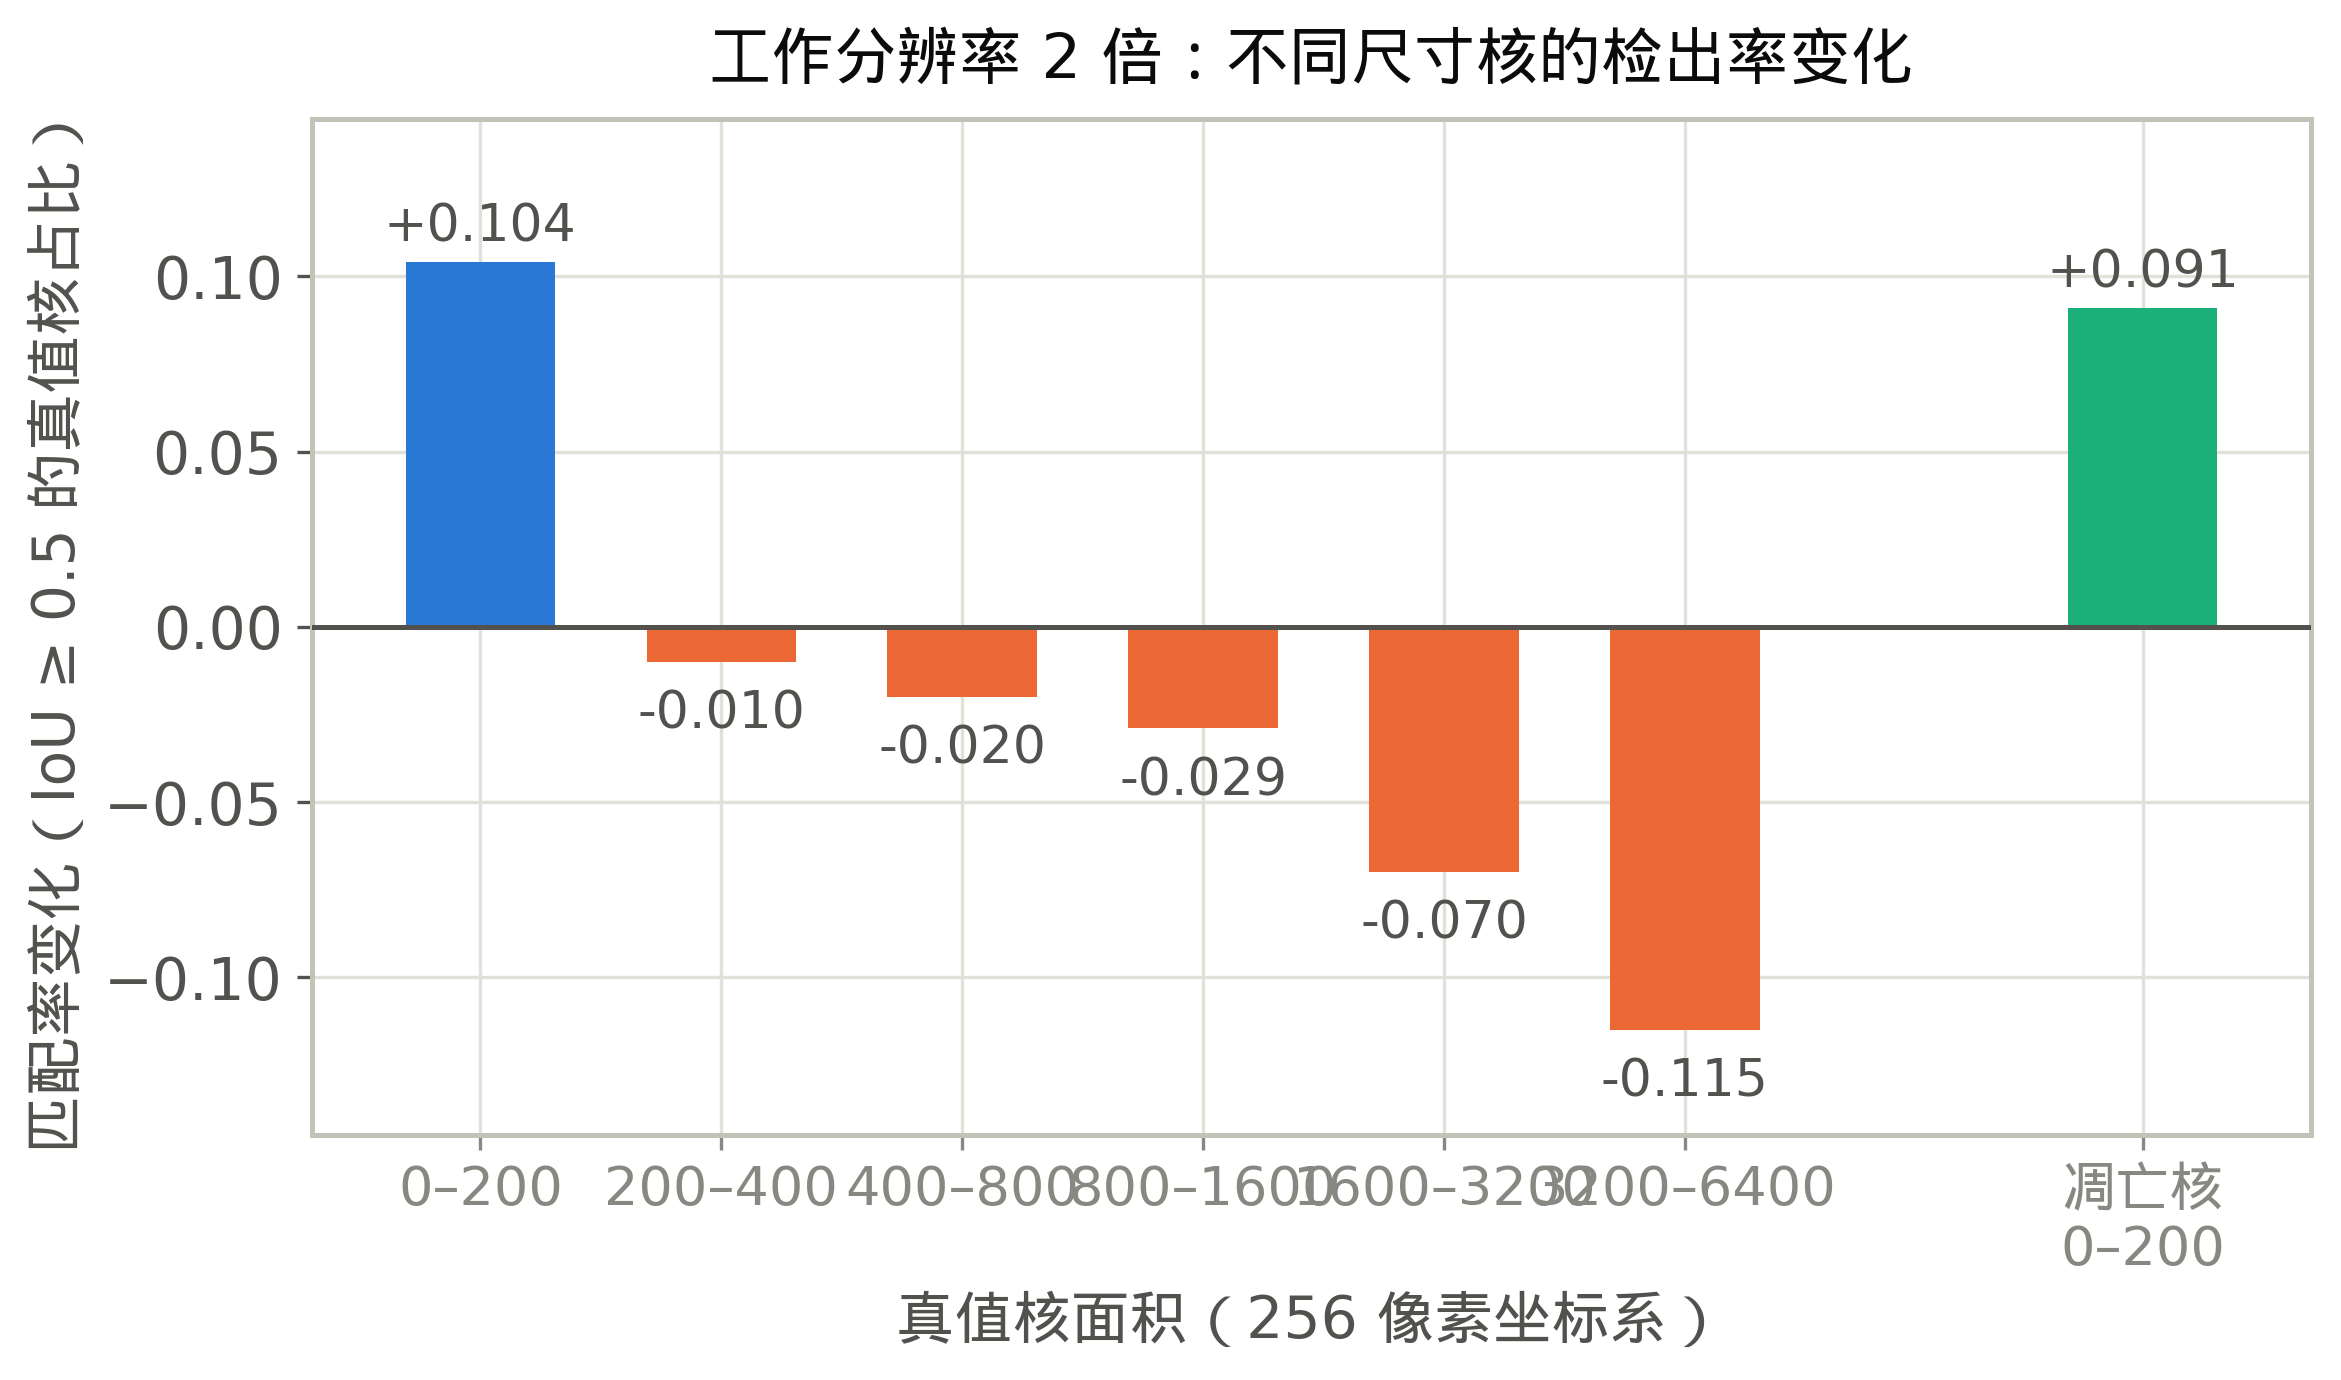
\includegraphics[width=0.88\linewidth]{figs/chart_size_bins_zh.png}
\caption{$2\times$ 分辨率带来的匹配率变化，按真值核面积分层（分裂 1 TTA，x2 种子 19 减
3 种子基线均值；IoU $\geq$ 0.5）。效应是\emph{尺寸}的单调函数，与类别无关：200\,px 以下的
核全部获益（含 Dead，$+$.091），400\,px 以上的尺寸段全部受损，单调递减。每个尺寸段内匹配
对的 IoU 持平（$\pm$.01）。}
\label{fig:sizebins}
\end{figure}

\begin{figure}[t]
\centering
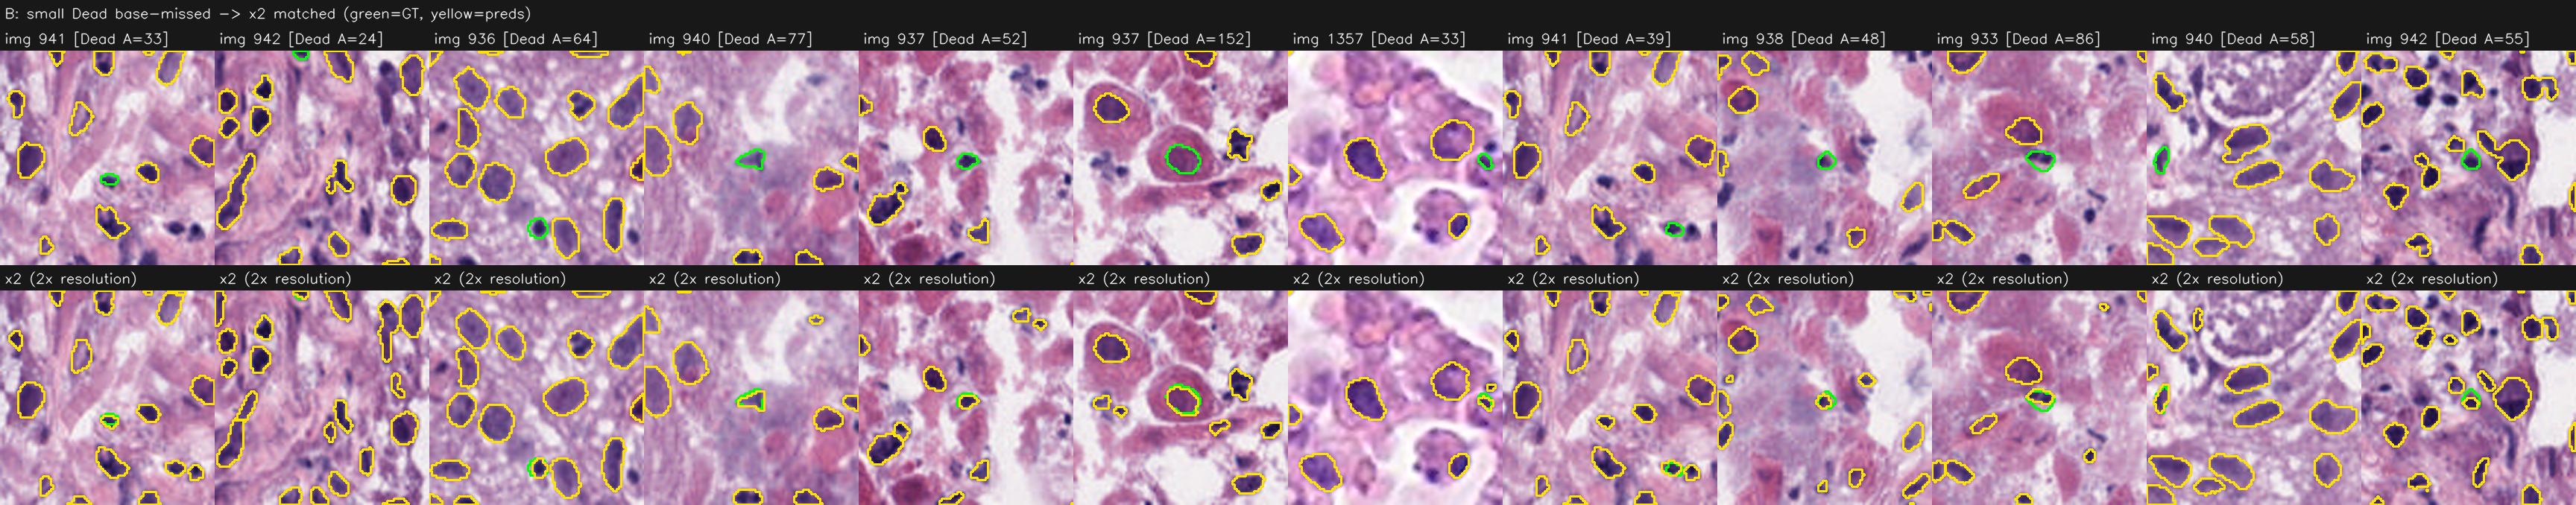
\includegraphics[width=\linewidth]{figs/x2_montage_gain.png}\\[2pt]
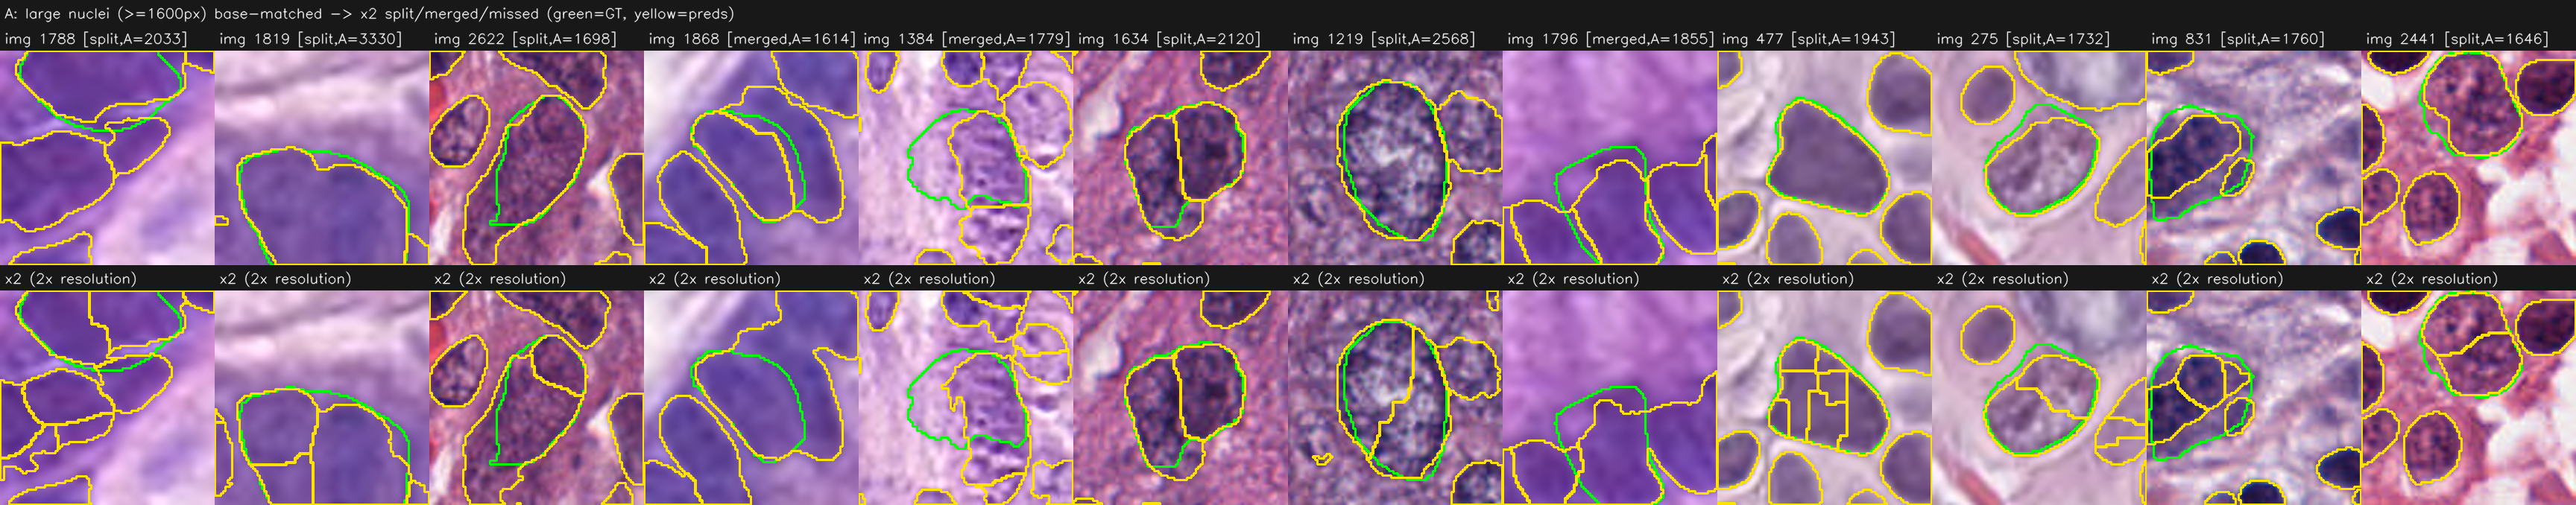
\includegraphics[width=\linewidth]{figs/x2_montage_damage.png}
\caption{上（增益）：256 下漏检的 Dead/小核（每对上排：无预测轮廓）在 512 下被检出（下
排）；绿色为真值轮廓，黄色为预测实例。下（损伤）：256 下作为单一实例匹配的大核（单轮廓）
在 512 下碎成内部马赛克——一个绿环内多个黄环——而外边界仍贴着真值。}
\label{fig:montage}
\end{figure}

三个观察定位了机制（图~\ref{fig:sizebins}--\ref{fig:montage}）：

\begin{enumerate}
\item \textbf{税与 Dead 增益不在同一处。}在 97 张含 Dead 的测试图上，
corr($\Delta$Dead, $\Delta$bPQ) $=+$.23；Dead 获益的图 bPQ 中性（$\Delta$bPQ 中位数
$+$.003），无 Dead 获益的图扛下损失（中位数 $-$.027）。这直接排除了"Dead 的改善蚕食了
其它类"。
\item \textbf{尺寸而非类别才是坐标轴。}200\,px 以下的非 Dead 核匹配率 $+$.104（Dead
0--200：$+$.091），随尺寸单调下滑至 3200--6400\,px 的 $-$.115。\emph{匹配对}的边界质量
不变（每个尺寸段 IoU $\pm$.01），核不是被匹配得更差——大核被\emph{切成了碎块}。误差构成
证实：GT split 率各类约翻倍（Neoplastic .009$\to$.017、Connective .013$\to$.025、Dead
.010$\to$.026）；大核（$\geq$1600\,px）非 Dead 中 split .072$\to$.104、merged
.003$\to$.009、missed-bg .024$\to$.054；每图预测实例数 25.5$\to$28.4，预测中 80\,px 以
下占比增至三倍（.034$\to$.109）；预测侧 fp-split 约翻倍（三个种子合并统计
.019$\to$.037）。拼接
图视觉审查：抽样的 12 个受损大核中 11 个是内部碎裂马赛克（单核最多碎成 7 块）而外轮廓仍
贴真值；抽样的 12 个小 Dead 增益全部是真实检出（平均 IoU 0.70）。
\item \textbf{显然的解释是错的。}"512$\to$256 的实例图最近邻降采样毁掉了边界"被每个尺寸
段的匹配 IoU 持平否定。真正的原因在解码里：HoVer-Net 后处理对预测图施加\emph{固定的像素
单位常数}——blob 与 marker 图上的 \texttt{remove\_small\_objects(min\_size=10)}（面积单位；
$2\times$ 下等效 2.5 原生 px$^2$），HV 图上孔径 $k{=}21$ 的 Sobel 算子（10.5 原生 px）。
分辨率倍增后，这些阈值在原生单位上一齐\emph{放松}：虚假 marker 在染色质纹理上存活并把大
核切碎，微小 blob 越过面积下限涌入预测集。而小核检测增益是真实的模型分辨率收益。
\end{enumerate}

\subsection{预注册解码修复（$du2$）}
\label{sec:du2}

修复方案由诊断直接给出，并在运行前注册：把像素单位常数按分辨率因子 $u$ 缩放——
$\mathrm{min\_size} \to 10u^2$，Sobel 孔径 $\to$ 最接近 $21u$ 的奇数（41）。（OpenCV 的
Sobel 孔径上限为 31；超过后我们对官方 21 抽头算子的脉冲响应核做线性重采样，$u{=}1$ 时严
格一致，已单元测试逐位一致。）对现有 checkpoint 重解码——不重训：

\begin{table}[t]
\centering\small
\caption{$du2$ 回收（3 分裂均值，种子 19，last checkpoint）。\% 为解码修复单独收回的
x2--基线差距占比。Dead 保住增益（且略有放大）。}
\label{tab:du2}
\begin{tabular}{llcccc}
\toprule
 & 手臂 & mPQ & bPQ & mPQ$^+$ & Dead PQ \\
\midrule
\multirow{3}{*}{无 TTA}
 & 基线 256     & .4995 & .6653 & .5178 & .1760 \\
 & x2           & .4791 & .6413 & .5012 & .1816 \\
 & x2 $+$ du2   & .4894 & .6583 & .5157 & .1831 \\
\cmidrule{2-6}
 & 收回         & 50\% & 71\% & 87\% & （增益扩大） \\
\midrule
\multirow{3}{*}{TTA}
 & 基线 256     & .5047 & .6706 & .5227 & .1767 \\
 & x2           & .4848 & .6488 & .5070 & .1786 \\
 & x2 $+$ du2   & .4926 & .6620 & .5189 & .1810 \\
\cmidrule{2-6}
 & 收回         & 39\% & 61\% & 76\% & （增益扩大） \\
\bottomrule
\end{tabular}
\end{table}

\begin{figure}[t]
\centering
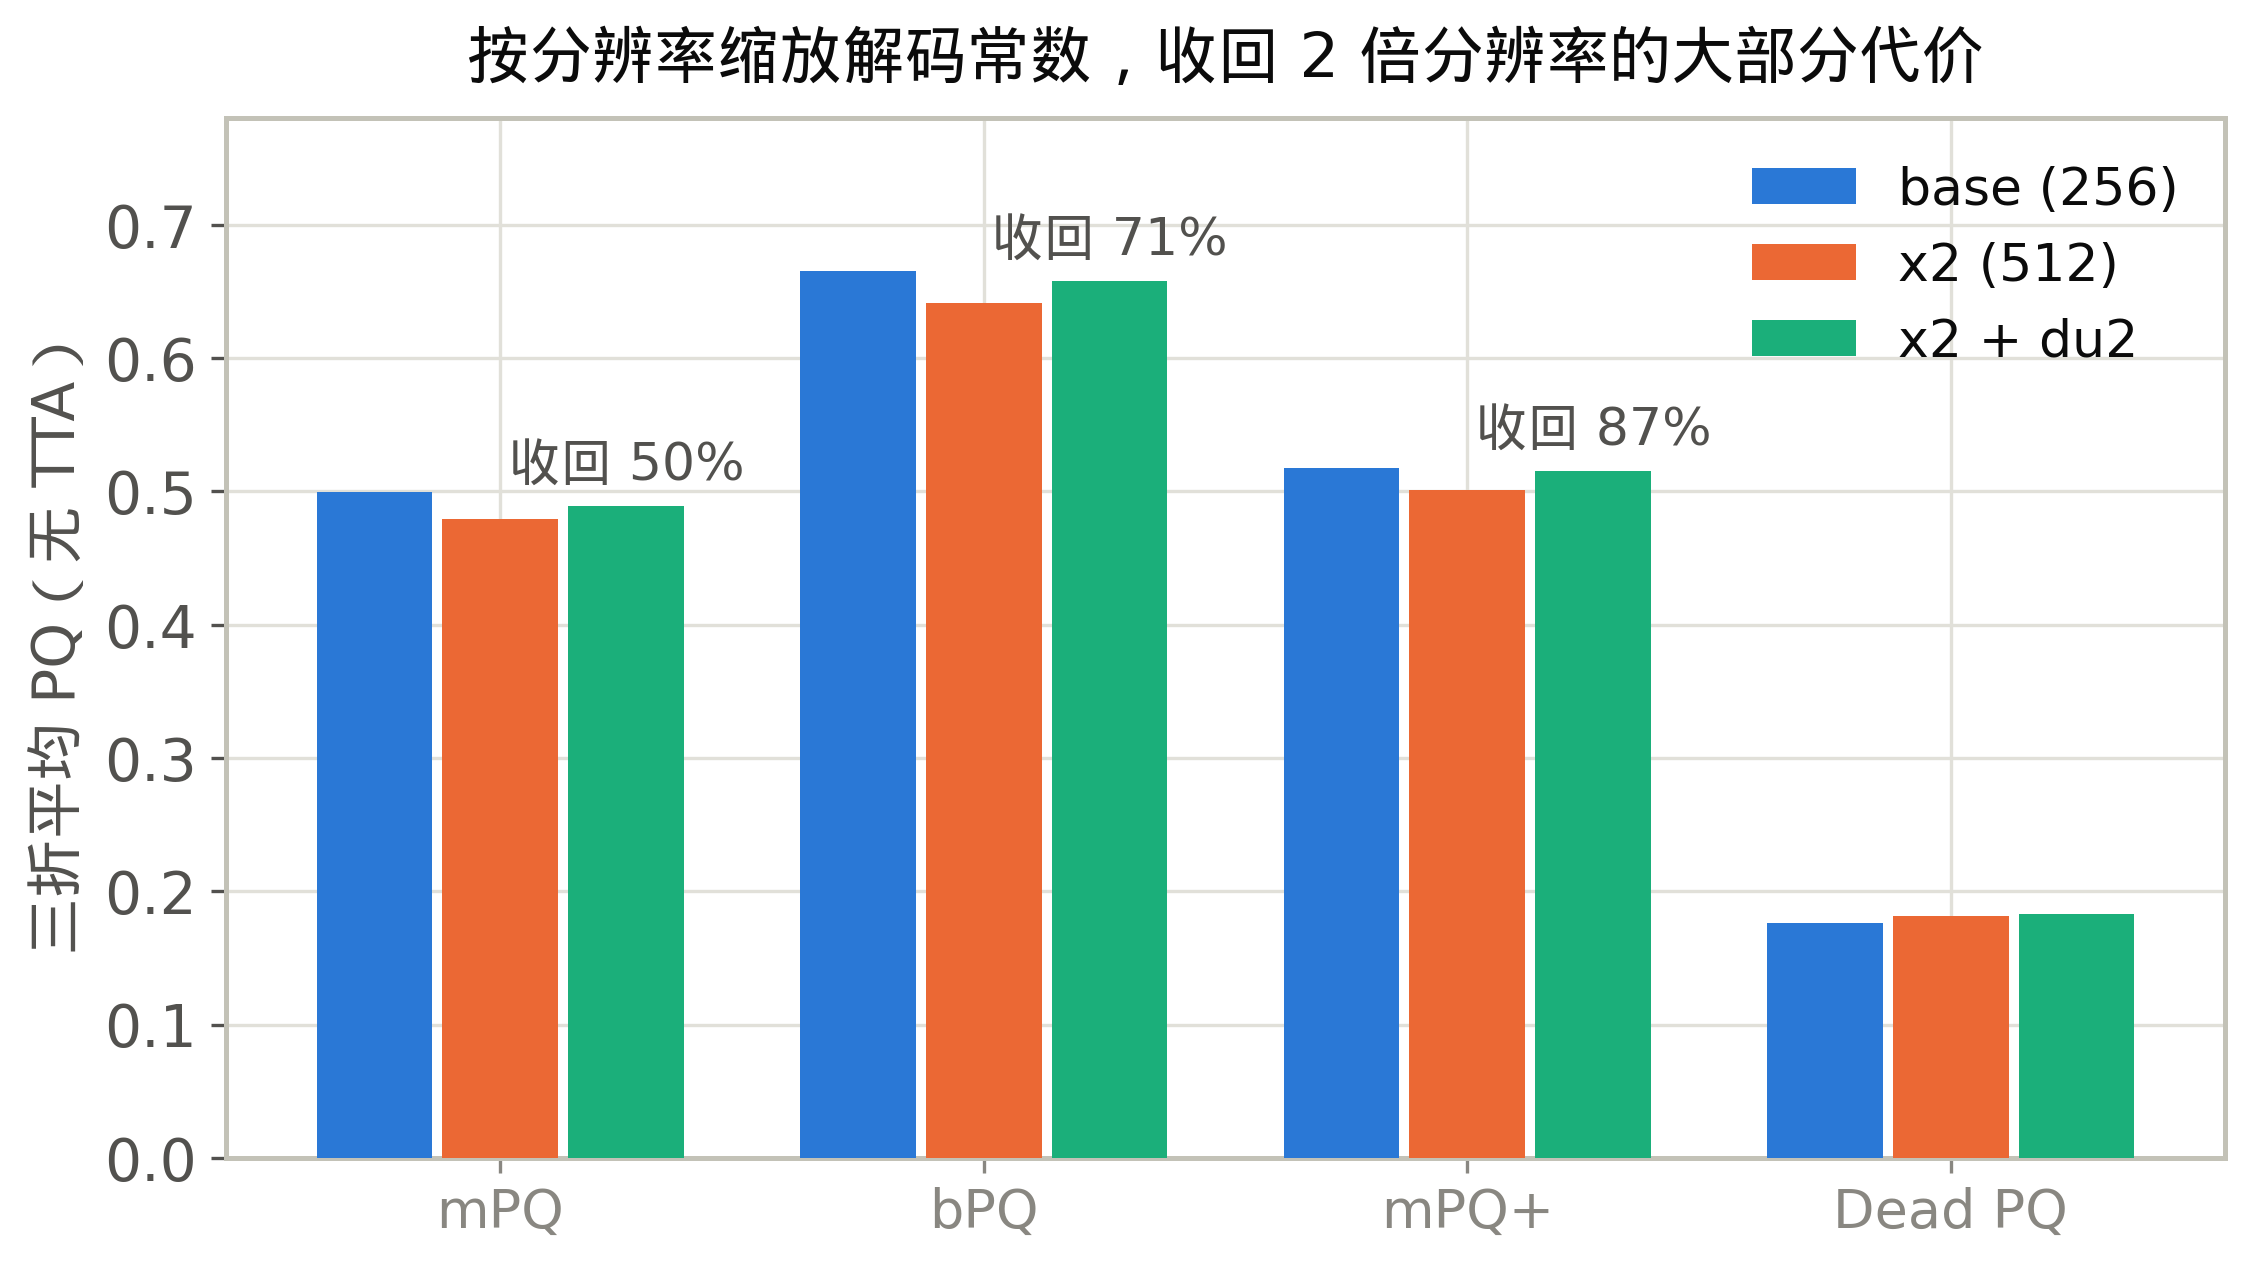
\includegraphics[width=0.86\linewidth]{figs/chart_du2_recovery_zh.png}
\caption{表~\ref{tab:du2}（无 TTA）：缩放两个解码常数即收回 $2\times$ 聚合代价的大部
分，同时 Dead 增益存活；mPQ$^+$ 与基线的差距缩到 .002 以内。}
\label{fig:du2}
\end{figure}

表~\ref{tab:du2}/图~\ref{fig:du2}：两个常数拥有这笔税的大头——依指标与 TTA 不同，占
mPQ/bPQ/mPQ$^+$ 代价的 50--87\%——且 Dead 增益保留并略有放大（无 TTA $+$.006$\to+$.007），
与机制的预测完全一致（边界质量本已持平；Dead 增益来自检测，而非解码）。逐分裂看，
x2 的 Dead 增益由折 3 驱动（分裂 1 $+$.017、分裂 2 $+$.009，无 TTA），分裂 3（测试折 1）
出现小幅损失（$-$.009），$du2$ 将其大部分收回（$-$.003）——与已知的 Dead 跨折组成差异
一致。残余差距（无 TTA bPQ $-$.007）是 512 下真实的 fp-split，不是解码问题：缩放第三个
常数（marker-open 核，$du2mk2$）在验证折上评估后\emph{未采纳}（bPQ 持平时 mPQ 更差）。

\subsection{仅验证折选择的杠杆：九个 run 上的严格改进}
\label{sec:lever}

对残余误差的视觉分析提示两个解码侧操作：合并相邻的同类实例（马赛克的外边界很干净），
丢弃贴边细条（微小 FP 中约三分之一是边界裁切片）。两者都有可调参数，且都只在\emph{验证
折}上、在 $du2$ 手臂上选择，规则为"bPQ $\geq$ 基线 $-$ .002，其次 mPQ 最大"。三个分裂的
验证扫描——加上第四次在解码变体上的扩展扫描——独立选出同一组参数：合并分数阈值 0.25，
细条面积下限 40\,px。

冻结后用于测试：

\begin{table}[t]
\centering\small
\caption{杠杆判定（$du2lev - du2$，配对图像 bootstrap 95\% CI）。上：最初三个分裂（种
子 19）。复现：$3{\times}3$ 网格全部 \textbf{9/9} 个 run 上 mPQ 与 bPQ 增量为正
（\S\ref{sec:grid}）；Dead 处处不变（CI 跨 0）。}
\label{tab:lever}
\begin{tabular}{lccc}
\toprule
分裂 & $\Delta$mPQ [CI] & $\Delta$bPQ [CI] & $\Delta$Dead PQ [CI] \\
\midrule
1 & $+$.0020 [$+$.0014, $+$.0026] & $+$.0030 [$+$.0022, $+$.0041] & $+$.0015 [$-$.0008, $+$.0051] \\
2 & $+$.0016 [$+$.0009, $+$.0022] & $+$.0025 [$+$.0018, $+$.0032] & $+$.0005 [$-$.0012, $+$.0028] \\
3 & $+$.0014 [$+$.0008, $+$.0021] & $+$.0021 [$+$.0014, $+$.0029] & $-$.0018 [$-$.0055, $+$.0016] \\
\bottomrule
\end{tabular}
\end{table}

表~\ref{tab:lever}：严格测试改进——六个 mPQ/bPQ CI 全部在正侧排除 0，所有 Dead 口径变
化在 $\pm$.002 内，每图预测实例 27.2$\to$26.6（杠杆只删掉每图约 0.5 个碎片与细条，别无可
测影响）。这一选择在完全不碰测试折的情况下完成了泛化。

\subsection{$3{\times}3$ 种子网格与预注册的种子噪声判定}
\label{sec:grid}

\begin{figure}[t]
\centering
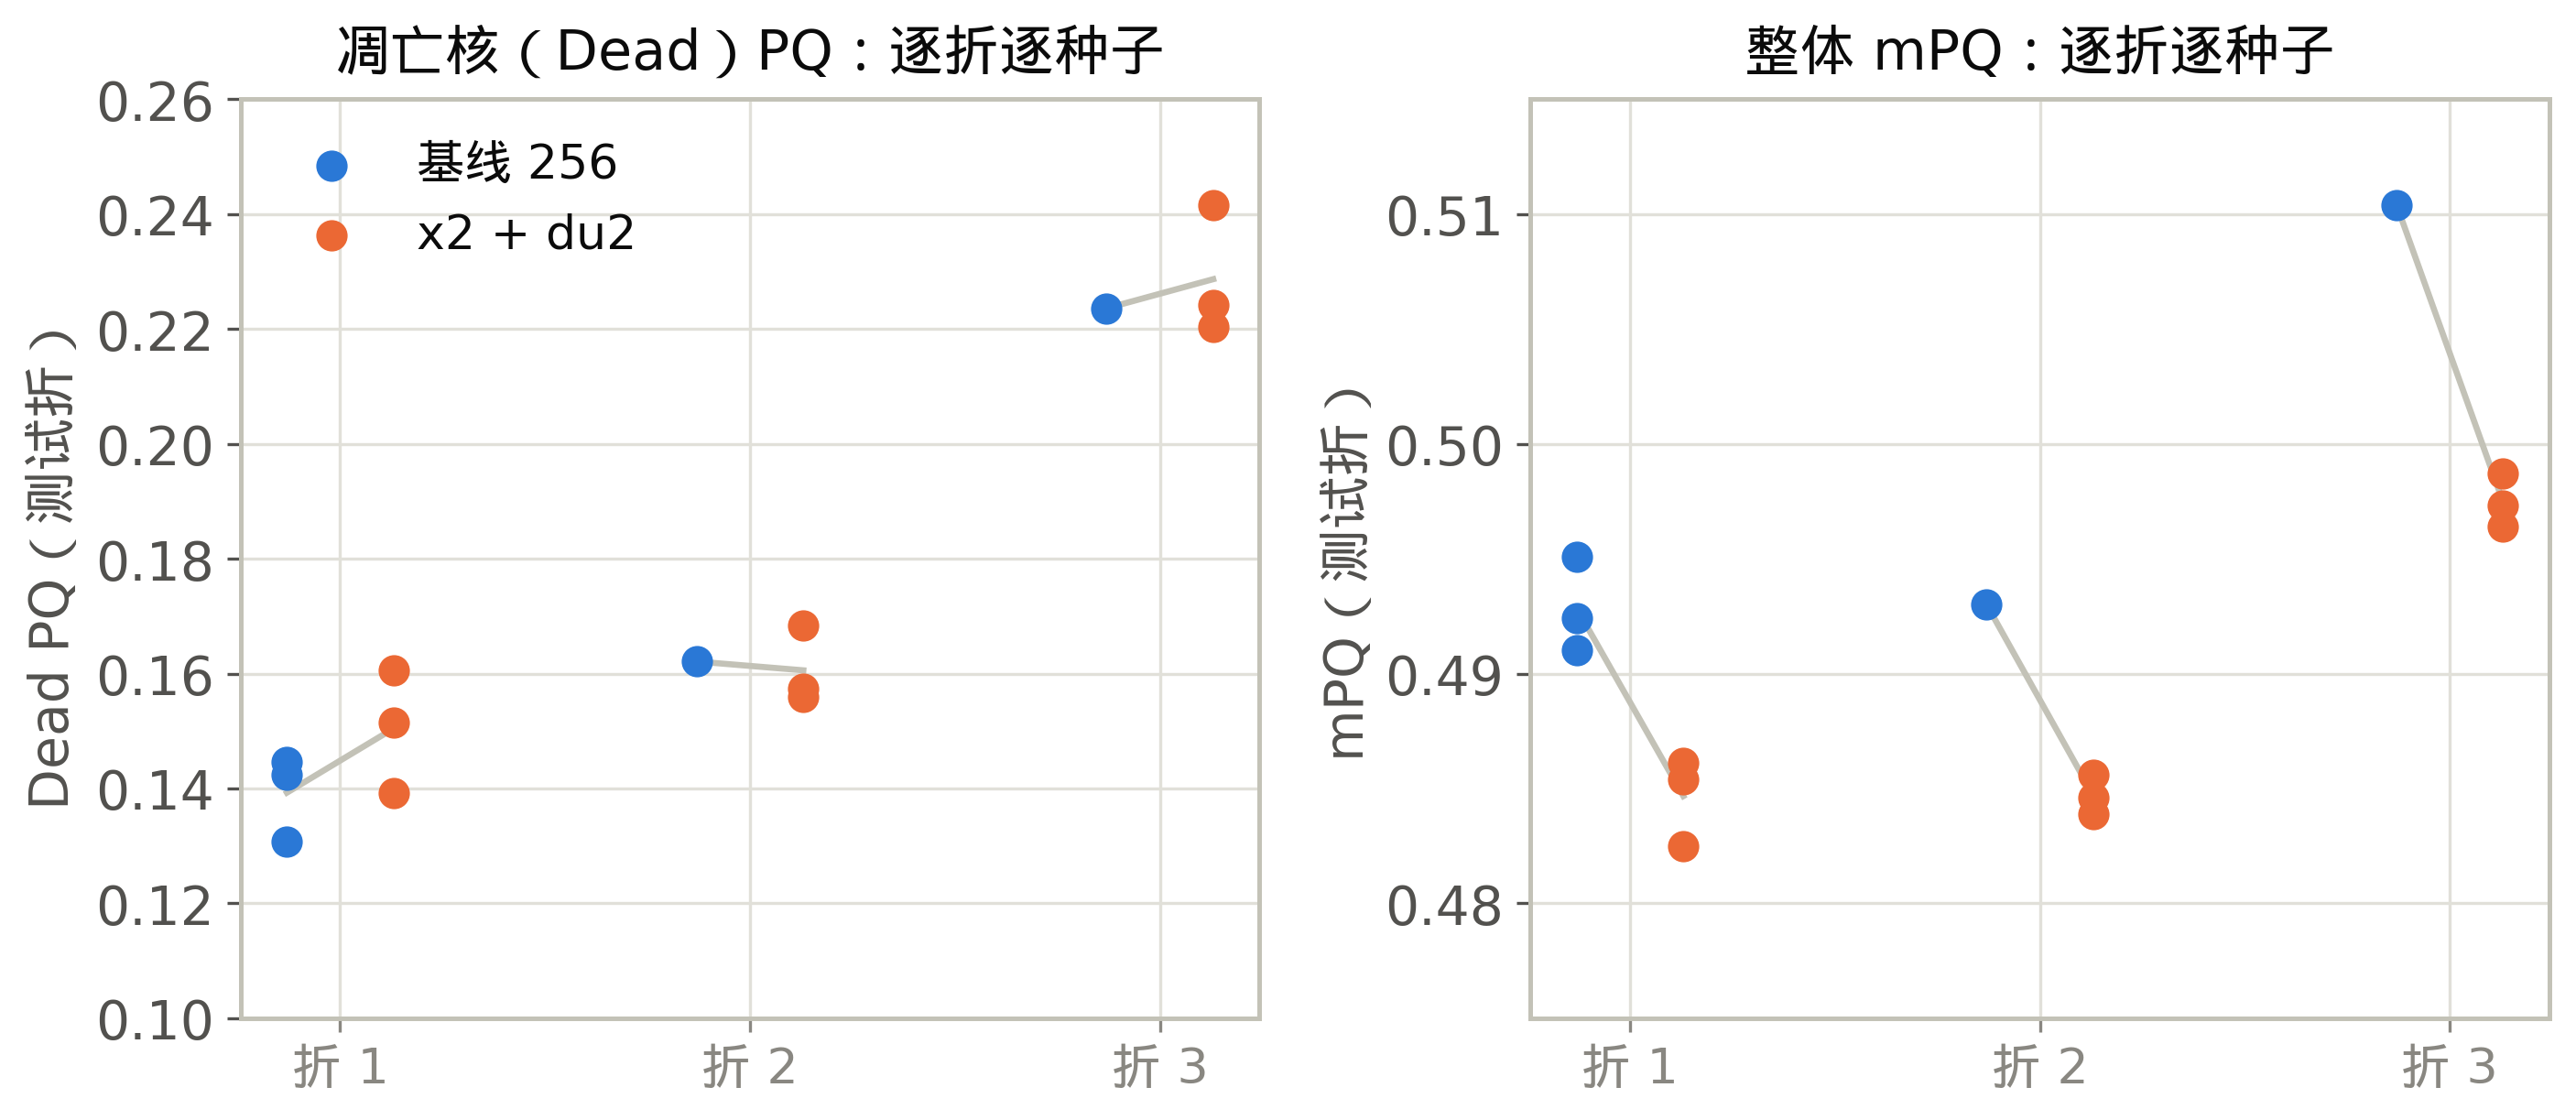
\includegraphics[width=0.98\linewidth]{figs/chart_seed_grid_zh.png}
\caption{种子网格。右：mPQ——每个分裂上全部 $du2$ run（橙）都低于基线 run（蓝），代价毫
无歧义。左：Dead PQ——run 相互交错；分裂 2 的 $du2$ 种子均值落在基线种子\emph{之下}，
分裂 3 的种子 19 翻号。连线为种子均值（基线额外种子只在分裂 1 存在）。}
\label{fig:grid}
\end{figure}

\begin{table}[t]
\centering\small
\caption{$3{\times}3$ 种子网格，逐分裂种子均值 $\pm$ 标准差（$du2$ 手臂；基线种子 1/2 仅
在分裂 1 存在）。下：种子均值的 3 分裂均值，及 $du2lev$ 手臂。}
\label{tab:grid}
\begin{tabular}{llccc}
\toprule
分裂 & 手臂 & mPQ & bPQ & Dead PQ \\
\midrule
\multirow{2}{*}{1} & 基线 & .4928 $\pm$ .0021 & .6661 $\pm$ .0015 & .1393 $\pm$ .0074 \\
                   & du2  & .4846 $\pm$ .0019 & .6565 $\pm$ .0003 & .1504 $\pm$ .0107 \\
\midrule
\multirow{2}{*}{2} & 基线 & .4930 & .6638 & .1621 \\
                   & du2  & .4847 $\pm$ .0009 & .6568 $\pm$ .0005 & .1606 $\pm$ .0068 \\
\midrule
\multirow{2}{*}{3} & 基线 & .5104 & .6647 & .2236 \\
                   & du2  & .4975 $\pm$ .0012 & .6605 $\pm$ .0013 & .2287 $\pm$ .0112 \\
\midrule
\multirow{3}{*}{3 分裂} & 基线   & .4987 & .6648 & .1750 \\
                        & du2    & .4889 & .6579 & .1799 \\
                        & du2lev & .4905 & .6603 & .1801 \\
\bottomrule
\end{tabular}
\end{table}

该网格（表~\ref{tab:grid}、图~\ref{fig:grid}）只有一个目的：预注册的种子噪声判
定——把 B 线的每个效应，对照同一配方逐种子训练的标准差。

\begin{itemize}
\item \textbf{代价是种子稳健的。}$\Delta$mPQ $-0.0098$ 与 $\Delta$bPQ $-0.0069$
（$du2$ 对基线，3 分裂均值）是最大逐分裂种子标准差（0.0021 / 0.0013）的 $4.7\times$ 与
$5.3\times$，9 个 run 全部同号。x1 在 mPQ/bPQ 上以约 $5\times$ 种子噪声的优势领先。
\item \textbf{Dead 增益是脆弱的。}3 分裂均值 $+$.0049 仅为逐种子 Dead 标准差
（0.0068--0.0112）的 $0.4$--$0.7\times$。同种子配对比较 5 组中 4 组有利于 $du2$（分裂 3
种子 19 变号，$-$.0032），分裂级种子均值为 $+$.0111（分裂 1，3/3 种子）/ $-$.0015（分裂
2，变号）/ $+$.0051（分裂 3，2/3）。x2 的 Dead 优势在分裂 1 上真实，分裂 3 上存在但噪声
大，分裂 2 上是平手。
\end{itemize}

\subsection{终局：明码标价的交换}
\label{sec:final}

表~\ref{tab:arch} 下块汇总终局（3 分裂均值，种子 19，无 TTA）：带杠杆的 $2\times$ 手臂以
$-$.0085 mPQ / $-$.0045 bPQ 换取内部 Dead 漏检 $-$.070（$0.372\!\to\!0.302$）、Dead
$F_c$ $+$.034、Dead DQ$^+$ $+$.026、去 Uterus Dead PQ $+$.009 与内部 Dead 匹配占比
$+$.07；mPQ$^+$ 持平（合并网格 $-$.0005；种子 19 $-$.0007）。按预注册联合端点，配合修正
解码的 $2\times$ 工作分辨率\textbf{不是默认的胜利}——它是一次明码标价的交换，且价格已全
部入账：解码常数（$du2$）约占 bPQ 税的三分之二，杠杆再收八分之一，残余约等于 512 下真实
的 fp-split。

\section{讨论}
\label{sec:discussion}

\paragraph{检测优先为何救不了 Dead。}A 线的两个结果形状相同。KongNet 的检测器找得到 Dead
核（逐核 $F_c$ 中游），但它的解码把相触的同类核并在一起，而 Dead 的失败几何恰恰是相触的
同类簇；LKCell-L 分离与匹配实例更好（bPQ、mPQ$^+$、Dead $F_c$ 全升），但检出的 Dead 核过
不了类型配对，检测增益变不成 Dead PQ。与报告一的负结果合起来，图景是：Dead 缺陷不属于某
个解码器家族，匹配协议下也没有任何已发表架构将它解决。真正能推动它的是分辨率——给小核
更多像素——但即便如此，改善的也只是检测，检出之后的分离与分型仍交由原来那套机器。

\paragraph{像素单位常数是一等混淆变量。}$du2$ 的意义超出本项目：所有建立在 HoVer-Net 后
处理之上的管线（几乎就是整个领域）都携带着按分辨率硬编码的常数。任何分辨率、图块尺寸或
backbone 步长改动都会悄然重缩放有效解码；未加修正的已发表分辨率消融，测到的是"改动
\emph{加上}一个偏向低分辨率的伪影"。我们在细胞核分割文献中未找到对此的讨论；两行的修复
已并入我们的解码器。

\paragraph{预注册的诚实效应量。}种子网格把经得起合并的与经不起的分开。代价以约
$5\times$ 种子噪声、统一符号存活；Dead PQ 增益作为头条数字根本经不起（$0.4$--$0.7\times$
种子标准差，一个分裂变号）。Dead 一侧真正坚实的是检测几何端点——内部 Dead 漏检 $-$.070
与 Dead $F_c$ $+$.034，逐 run 复现同号——而对 65--97 张含 Dead 图像做的类 PQ 聚合，仍是
该基准里噪声最大的测量。这正是报告一的噪声标定在起作用：不该信的是头条数字，我们说清了
该信哪个。

\paragraph{评测配方，老问题。}LKCell-L 是继报告一 HoVer-NeXt-T 之后第二个发布数字超出我们
严格复评超过排行榜典型间距（均匀约 0.015）的模型，而 KongNet 的头条 Dead 优势在验证折调
优解码下干脆不复现。两个差距都是协议而非管线：配方一旦对齐，一切都干净复现。排行榜的有
意义分辨率，比它的配方还细。

\section{状态与后续工作}
\label{sec:status}

A 线与 B 线均已完成并关闭（A 负结果；B 为机制清楚、全复现的明码标价交换）。最终报告之前
剩余：复评其余发布分折权重（PromptNucSeg、CellVTA），把跨域 rank 池从四个架构扩到六个；
最终报告的图组（组织$\times$类别热力图、跨架构误差分解）；可选的额外外部集（MoNuSeg、
NuInsSeg）；以及尚未启动的 phase-2 数据方向（更大规模无泄漏训练数据、外部 Dead 标签池
化）——它是分辨率之外 Dead 问题最主要的待开杠杆。

\begin{thebibliography}{99}\small
\bibitem{gamper2019pannuke} J.~Gamper, N.~Alemi~Koohbanani, K.~Benet, A.~Khuram, N.~Rajpoot,
``PanNuke: An Open Pan-Cancer Histology Dataset for Nuclei Instance Segmentation and
Classification,'' \emph{ECDP}, LNCS 11435, pp.~11--19, 2019; and J.~Gamper et al., ``PanNuke
Dataset Extension, Insights and Baselines,'' arXiv:2003.10778, 2020.
\bibitem{graham2019hovernet} S.~Graham, Q.~D.~Vu, S.~E.~Raza, A.~Azam, Y.-W.~Tsang,
J.~Kwak, N.~Rajpoot, ``HoVer-Net: Simultaneous Segmentation and Classification of Nuclei in
Multi-Tissue Histology Images,'' \emph{Medical Image Analysis}, 58:101563, 2019.
\bibitem{horta2024cellvit} F.~H\"orst, M.~Rempe, L.~Heine, J.~Kleesiek, ``CellViT: Vision
Transformers for Precise Cell Segmentation and Classification,'' \emph{Medical Image
Analysis}, 94:103143, 2024.
\bibitem{horta2025cellvitpp} F.~H\"orst, M.~Rempe, H.~Becker, L.~Heine, J.~Keyl, J.~Kleesiek,
``CellViT++: Energy-Efficient and Adaptive Cell Segmentation and Classification Using
Foundation Models,'' \emph{Computer Methods and Programs in Biomedicine}, 277:109206, 2026.
\bibitem{hovenext} E.~Baumann, B.~Dislich, J.~L.~Rumberger, J.~L.~Nagtegaal,
M.~Rodr\'iguez~Mart\'inez, I.~Zlobec, ``HoVer-NeXt: A Fast Nuclei Segmentation and
Classification Pipeline for Next Generation Histopathology,'' \emph{MIDL}, PMLR 250:61--86,
2024.
\bibitem{promptnucseg} Z.~Shui, Y.~Zhang, K.~Yao, C.~Zhu, S.~Zheng, J.~Li, H.~Li, Y.~Sun,
R.~Guo, L.~Yang, ``Unleashing the Power of Prompt-Driven Nucleus Instance Segmentation
(PromptNucSeg),'' \emph{ECCV}, LNCS 15085, pp.~288--304, 2024.
\bibitem{lv2025kongnet} J.~Lv, E.~S.~Nasir, K.~Xu, M.~Jahanifar, B.~S.~Chohan,
B.~Elhaminia, S.~E.~A.~Raza, ``KongNet: A Multi-headed Deep Learning Model for Detection and
Classification of Nuclei in Histopathology Images,'' arXiv:2510.23559, 2025.
\bibitem{cui2024lkcell} Z.~Cui, J.~Yao, L.~Zeng, J.~Yang, W.~Liu, X.~Wang, ``LKCell:
Efficient Cell Nuclei Instance Segmentation with Large Convolution Kernels,''
arXiv:2407.18054, 2024.
\end{thebibliography}

\end{document}
